\documentclass[10pt,letterpaper]{article}
\usepackage{fontspec}
\usepackage{amsmath,amssymb}
\usepackage{graphicx}
\usepackage{xcolor}
\usepackage{tcolorbox}
\tcbuselibrary{skins}
\usepackage{geometry}
\usepackage{booktabs}
\usepackage{colortbl}
\usepackage{fancyhdr}
\usepackage{titlesec}
\usepackage[shortlabels,inline]{enumitem}
\usepackage{tabularx}
\usepackage{array}
\usepackage{multicol}
\usepackage{tikz}

\setmainfont{Times New Roman}
\setsansfont{Arial}

\geometry{
    paperwidth=612.05pt,
    paperheight=720.05pt,
    top=20pt,
    headheight=14pt,
    headsep=12pt,
    bottom=28pt,
    footskip=12pt,
    left=36pt,
    right=36pt
}

\definecolor{stewartcyan}{RGB}{0, 118, 186}
\definecolor{stewartred}{RGB}{218, 41, 28}
\definecolor{stewarttableheader}{RGB}{210, 224, 238}
\definecolor{stewarttablehead}{RGB}{210, 224, 238}
\definecolor{tableblue}{RGB}{210, 224, 238}
\definecolor{stewartlightblue}{RGB}{235, 243, 250}
\definecolor{stewartblue}{RGB}{0, 118, 186}
\definecolor{stewartgray}{RGB}{120, 120, 120}
\definecolor{stewartlightgray}{RGB}{240, 240, 240}
\definecolor{stewartpurple}{RGB}{85, 30, 95}
\definecolor{stewartpurplebg}{RGB}{243, 238, 245}
\definecolor{stewartpurpletext}{RGB}{85, 30, 95}
\definecolor{darkgray}{RGB}{40, 40, 40}

\pagestyle{fancy}
\fancyhf{}
\renewcommand{\headrulewidth}{0pt}

\providecommand{\makecell}[2][c]{\begin{tabular}[#1]{@{}c@{}}#2\end{tabular}}
\providecommand{\faDesktop}{\textbf{[Máy tính]}}
\providecommand{\casicon}{\textbf{\textsf{[CAS]}}}
\providecommand{\ticon}{\textbf{\textsf{[T]}}}
\providecommand{\captionof}[2]{\par\vspace{2pt}{\small\textbf{#1}: #2}\par}
\NewDocumentEnvironment{tasks}{o d()}{\begin{enumerate}}{\end{enumerate}}
\providecommand{\task}{\item}
\newenvironment{redframebox}{\begin{definitionbox}}{\end{definitionbox}}

\newtcolorbox{definitionbox}{
    colback=white,
    colframe=stewartred,
    arc=0mm,
    boxrule=0.9pt,
    left=3.5mm, right=3.5mm, top=3mm, bottom=3mm
}

\begin{document}

\setlength{\abovedisplayskip}{3pt}
\setlength{\belowdisplayskip}{3pt}
\setlength{\abovedisplayshortskip}{1pt}
\setlength{\belowdisplayshortskip}{1pt}
\fancyhead[L]{\textbf{\large 8}\quad\sffamily\textbf{\color{darkgray}CHƯƠNG 1}\quad\sffamily\color{darkgray}Hàm số và Mô hình}
\fancyhead[R]{}

\noindent
\begin{minipage}[t]{0.26\textwidth}
    \vspace{3.75cm}
    {\small\textbf{\textsf{Bảng 1}}\quad \textsf{Dân số thế giới}}\\[0.15cm]
    \small
    \begin{tabular}{|c|c|}
        \hline
        \rowcolor{stewarttableheader}
        \textbf{Năm} & \textbf{\shortstack{Dân số\\(triệu người)}} \\
        \hline
        1900 & 1650 \\
        1910 & 1750 \\
        1920 & 1860 \\
        1930 & 2070 \\
        1940 & 2300 \\
        1950 & 2560 \\
        1960 & 3040 \\
        1970 & 3710 \\
        1980 & 4450 \\
        1990 & 5280 \\
        2000 & 6080 \\
        2010 & 6870 \\
        \hline
    \end{tabular}

    \vspace{3.35cm}
    {\raggedleft
    {\small\textbf{\textsf{HÌNH 1}}}\\[2pt]
    {\footnotesize Gia tốc thẳng đứng của mặt đất trong trận động đất Northridge}\par}
\end{minipage}%
\hfill
\begin{minipage}[t]{0.71\textwidth}
    \noindent
    \parbox[c]{1.5cm}{%
        \color{stewartcyan}%
        \rule{1.5cm}{0.6pt}\\[2.2pt]%
        \rule{1.5cm}{0.6pt}\\[2.2pt]%
        \rule{1.5cm}{0.6pt}\\[2.2pt]%
        \rule{1.5cm}{0.6pt}\\[2.2pt]%
        \rule{1.5cm}{0.6pt}%
    }%
    \hspace{0.25cm}%
    {\color{stewartcyan}\LARGE\textbf{\textsf{1.1}}}%
    \hspace{0.25cm}%
    {\color{stewartcyan}\rule[-0.2cm]{0.8pt}{0.85cm}}%
    \hspace{0.25cm}%
    {\LARGE\textbf{\textsf{Bốn cách biểu diễn một hàm số}}}
    
    \vspace{0.4cm}
    \noindent{\large\textbf{\textsf{\color{stewartcyan}■ Hàm số}}}
    \vspace{0.18cm}

    Hàm số xuất hiện bất cứ khi nào một đại lượng này phụ thuộc vào một đại lượng khác. Hãy xem xét bốn tình huống sau:

    \begin{description}[leftmargin=1.5em, itemsep=1pt, topsep=2pt, partopsep=0pt, parsep=0pt]
        \item[\textbf{A.}] Diện tích $A$ của một hình tròn phụ thuộc vào bán kính $r$ của hình tròn đó. Mối liên hệ giữa $r$ và $A$ được xác định bởi công thức $A = \pi r^2$. Ứng với mỗi số dương $r$, ta luôn xác định được duy nhất một giá trị $A$ tương ứng, và ta nói rằng $A$ là một \textit{hàm số} của $r$.

        \item[\textbf{B.}] Dân số thế giới $P$ phụ thuộc vào thời gian $t$. Bảng 1 cung cấp số liệu ước tính về dân số thế giới $P$ tại các mốc thời gian $t$ trong một số năm nhất định. Chẳng hạn:
        \[
        P \approx 2{,}560{,}000{,}000 \quad \text{khi } t = 1950
        \]
        Ứng với mỗi giá trị của thời gian $t$, luôn có một giá trị tương ứng của $P$, và ta nói rằng $P$ là một hàm số của $t$.

        \item[\textbf{C.}] Cước phí bưu điện $C$ để gửi một phong bì phụ thuộc vào trọng lượng $w$ của nó. Dù không có một công thức toán học đơn giản nào biểu diễn trực tiếp mối quan hệ giữa $w$ và $C$, bưu điện vẫn có một bảng quy tắc rõ ràng để xác định giá trị của $C$ khi biết trước $w$.

        \item[\textbf{D.}] Gia tốc thẳng đứng $a$ của mặt đất đo được bởi một địa chấn kế trong suốt một trận động đất là một hàm số theo thời gian trôi qua $t$. Hình 1 thể hiện đồ thị ghi lại hoạt động địa chấn trong trận động đất Northridge làm rung chuyển Los Angeles vào năm 1994. Với một giá trị thời gian $t$ cho trước, đồ thị cung cấp cho ta một giá trị gia tốc $a$ tương ứng.
    \end{description}

    \vspace{0.08cm}
    {\centering
        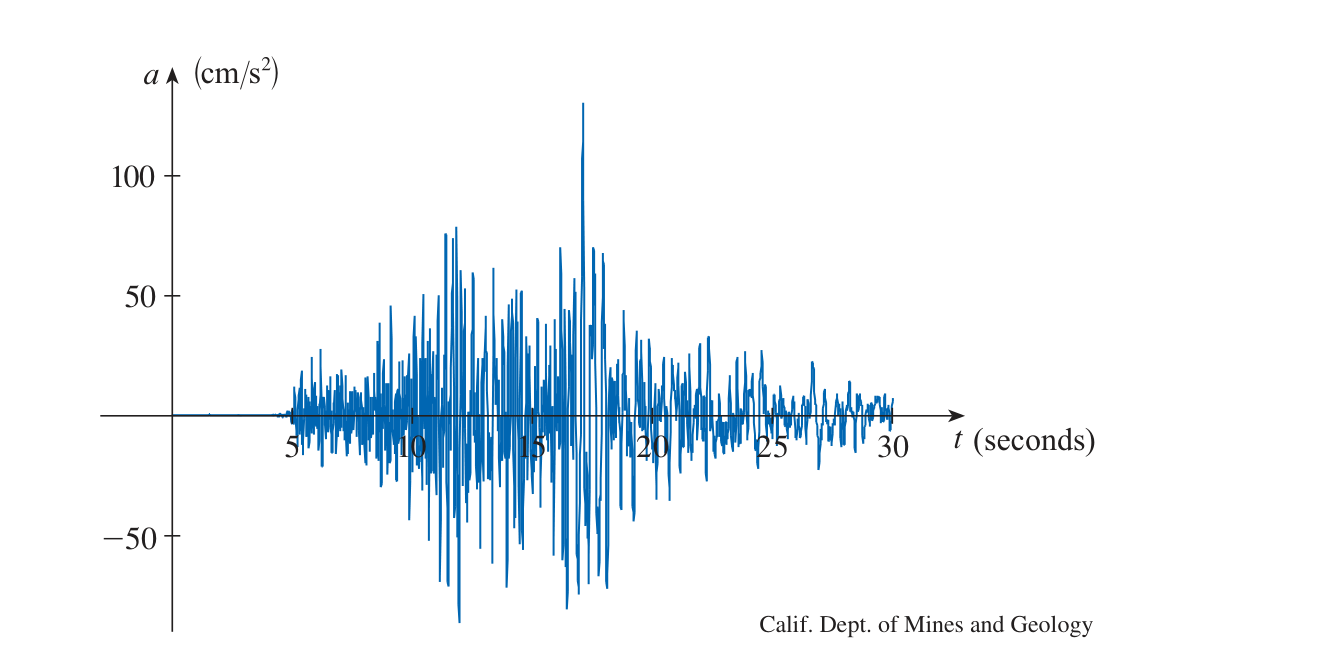
\includegraphics[width=0.88\linewidth]{images/figure_1_clean.png}
    \par}
    \vspace{-0.2cm}

    Mỗi ví dụ trên đều mô tả một quy tắc sao cho khi cho trước một số ($r$ trong Ví dụ A), một giá trị số khác ($A$) sẽ được xác định tương ứng. Trong mỗi trường hợp, ta nói rằng số thứ hai là một hàm số của số thứ nhất. Nếu dùng chữ cái $f$ để đại diện cho quy tắc liên hệ giữa $A$ và $r$ trong Ví dụ A, ta biểu diễn mối liên hệ này bằng \textbf{ký hiệu hàm số} là $A = f(r)$.

    \begin{definitionbox}
    Một \textbf{hàm số} $f$ là một quy tắc đặt tương ứng mỗi phần tử $x$ thuộc một tập hợp $D$ với duy nhất một phần tử, ký hiệu là $f(x)$, thuộc một tập hợp $E$.
    \end{definitionbox}

    Chúng ta thường khảo sát các hàm số mà các tập hợp $D$ và $E$ đều là tập hợp các số thực. Tập hợp $D$ được gọi là \textbf{tập xác định} (\textit{domain}) của hàm số. Số $f(x)$ được gọi là \textbf{giá trị của $f$ tại $x$} và được đọc là ``$f$ của $x$'' (hay ``$f$ tại $x$''). \textbf{Tập giá trị} (\textit{range}) của $f$ là tập hợp tất cả các giá trị có thể có của $f(x)$ khi $x$ biến thiên trên toàn bộ tập xác định.
\end{minipage}
\end{document}
